% !TeX root = main.tex
% !TeX spellcheck = de_DE
% !TeX encoding = utf8

\chapter{Flash Memory}
Flash memory often in the form of solid state drives (SSD) are becoming more and more of primary storage for computers. The cost per storage has been decreasing steadily therefore driving adoption. Especially the low access latency and the high possible throughput compared so spinning disk hard drives are an advantage. In the application predominantly NAND type flash is used due to its higher density. 


\section{Flash Basics}
NAND flash which will be discussed is of most interest for SSDs due to its high density and therefore lower cost per bit. \cref{fg_tans} shows a floating gate transistor which is used to store data. By inserting charge into the floating gate it is possible to change the threshold voltage of the transistor. Multiple of these floating gate transistor are connected in series to for a so called NAND string. In this nand string the drain and source neighboring transistors are connected to form a continuos string as seen in \cref{nand_string}. Also on the top is a normal bit line select transistor to connect the string to be read to a bit line. On the bottom is the ground select transistor to connect the string to ground\cite[p.~22-24]{MiMa18}.

\begin{figure}
    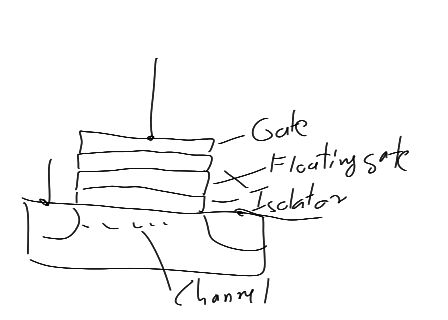
\includegraphics[width=5cm]{fg_schema.png}
    \centering
    \caption{A floating gate field effect transistor}
    \label{fg_tans}
\end{figure}


\begin{figure}
    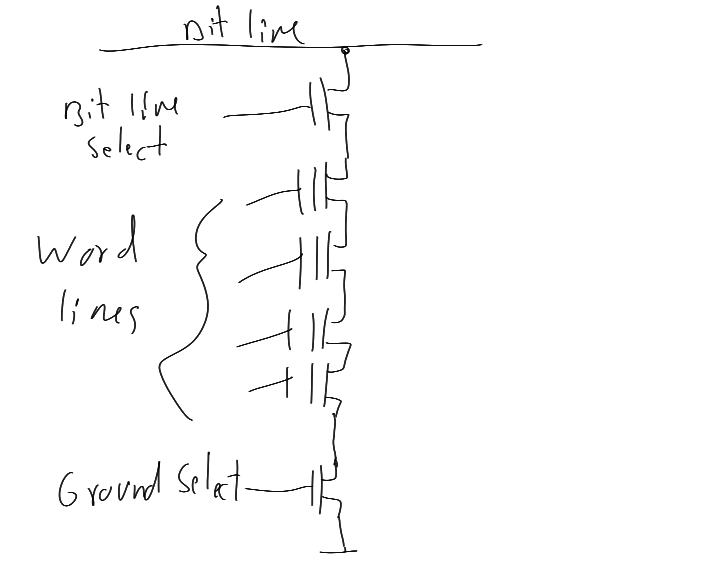
\includegraphics[width=5cm]{nand_schema.png}
    \centering
    \caption{Multiple transistors are arranged to make a NAND string}
    \label{nand_string}
\end{figure}

NAND Flash is arranged into blocks and pages. Due to its arrangement NAND memory can only be erased whole blocks at a time. Whereas each page can be programmed individually. When a cell is erased, in it considered "1". On the other hand when programmed it is "0". Programming is done by applying a high voltage to the control gate. This causes electrons from the channel to move through the lower oxide layer into the floating gate. The electrons are now trapped in the control gate under normal conditions. To erase a block the substrate for this block it raised to a high potential to pull the electrons back out of the floating gate\cite{RiTo98}.

\subsection{Reading}
To read a page the select word line is set at the read voltage. This read voltage is between the threshold voltage for a programmed and unprogrammed cell. Thus if the cell was programmed it will not conduct, on the other hand if it was unprogrammed the applied gate voltage is above the threshold voltage and the cell conducts. In \cref{nand_th} an example distribution for cell threshold voltages can be seen. The voltage at the bit line is measured using a read amplifier which then outputs the data. 

\begin{figure}
    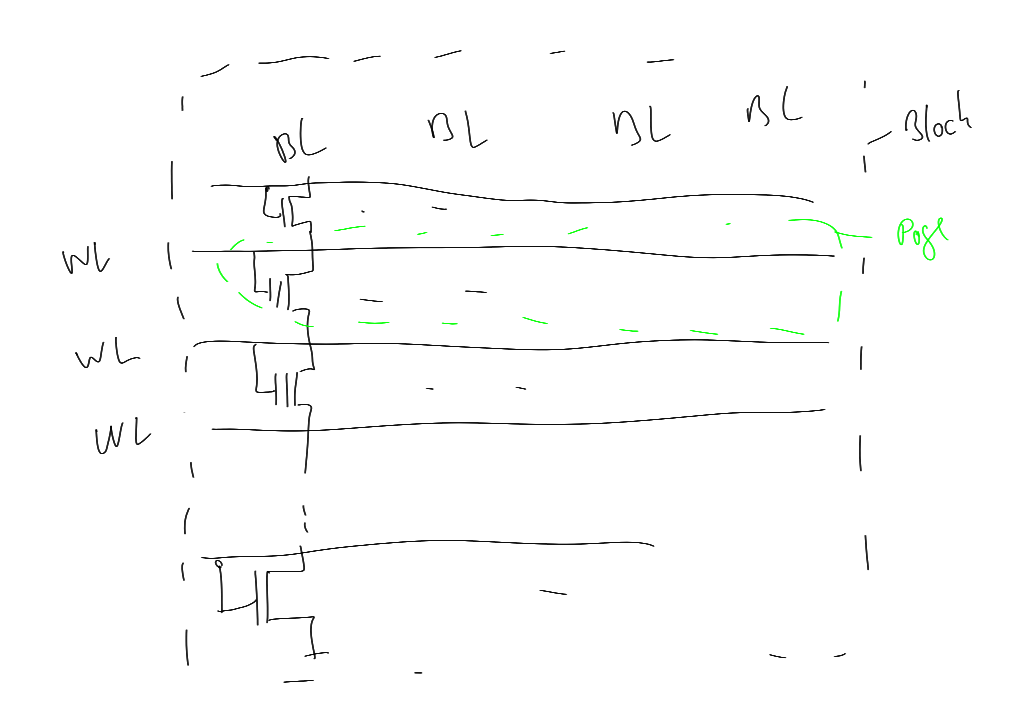
\includegraphics[width=5cm]{nand_array.png}
    \centering
    \caption{Array Organization of NAND memory}
    \label{nand_array}
\end{figure}

\subsection{Erasing}
Erasing is done by lifting the substrate voltage to to high potential while keeping the gate voltage low. This forces the electrons trapped inside the floating gate through the insulator into the substrate. As the charge is now removed from the gate the threshold voltage is reduced to the erased state. The erase is done a whole block built like \cref{nand_array} at a time.

\subsection{Programming}
When Programming the word line for the selected page is set to a high voltage. The bit lines where the cells should be programmed are kept at 0V. All other bit lines are set to high voltage to inhibit them. When the bit line is set to a high voltage the channel of the target cell is also at this voltage so the gate and channel are both at the hight potential.

\begin{figure}
    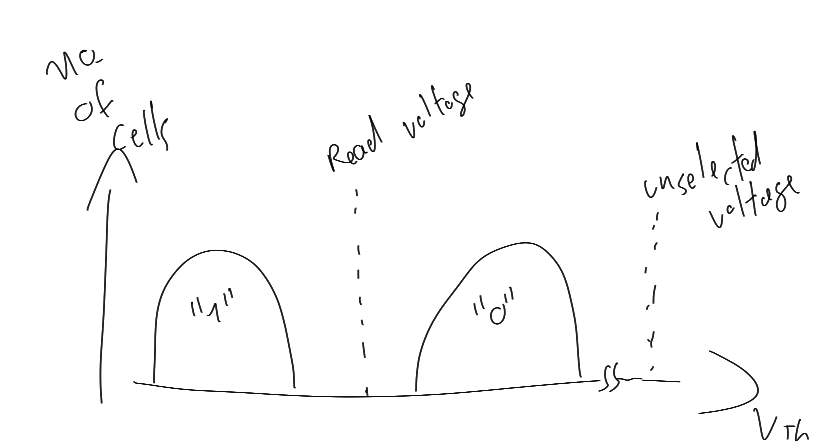
\includegraphics[width=5cm]{slc_vth_dist.png}
    \centering
    \caption{Threshold Distribution of a Floating Gate Transistor\cite{RiTo98}}
    \label{nand_th}
\end{figure}

\section{Error Types}


\cite{ZaTu16}